\documentclass{article}
\usepackage[utf8]{inputenc}
\usepackage{fancyhdr}
\usepackage[left=2cm,right=2cm,top=3cm,bottom=3cm]{geometry}
\usepackage{hyperref}
\usepackage{pdflscape}
\usepackage{pdfpages}
\usepackage{float}
\usepackage{multirow}
\usepackage{array}
\usepackage{longtable}
\usepackage{colortbl}
\usepackage{enumitem}


%\usepackage{xcolor}
\title{Router hardware| Plan of approach}
\author{Pieter ten Velde}
\date{September 2022}

%Page style
\pagestyle{fancy}
\fancyhf{}
\lhead{Plan of approach}
\rhead{Router}
\rfoot{Page \thepage}
\lfoot{\today}
\setlength{\headheight}{15pt}

\begin{document}
\setlist{nolistsep,leftmargin=*}
\maketitle
\newpage
\tableofcontents
\newpage

\newpage
\section{Project results}
\subsection{Background}
Crownstone, established in Rotterdam, Stationsplein 45 d1.118, https://crownstone.rocks, is a manufacturer of smart plugs and connections. Crownstone designs products like switches, dimmers, energy monitoring and soft fuses. Crownstone's technology aims to play an important role in the energy transition with a "smarter home". This can be done for example by playing in on the residents of the home(turning on lights or the heating when people are present), by getting a better insight into energy consumption or by using energy on smart moments. An excess of energy is often caused by sustainable energy sources like wind and solar energy. By limiting the excess of energy, a household will truly use the generated sustainable energy.
\subsection{Issue}
\label{subsub:probleemstelling}
The Crownstone hardware can be controlled from a smartphone. However the use of a smartphone means:
\begin{enumerate}
    \item no switching from a distance
    \item no continuous storage of the energy usage
    \item not for example, being able to react to changing electricity prices.
\end{enumerate}

By using a hub like a PI with an Crownstone dongle with Home Assistant from a Homey this becomes (partially) possible, but a lot of functionality stays absent.

\subsection{Objective}
Crownstone want to offer a router that has different features:
\begin{enumerate}
    \item direct Bluetooth Mesh support
    \item Long term energy storage
    \item Matter Border Router support
    \item connections 
    \begin{itemize}
        \item Ethernet (RJ45)
        \item smart meter(RJ11)
        \item Heat pumps/solar panels/charging stations(RS485, screw connector)
    \end{itemize}
\end{enumerate}
The router will be placed in a fuse box and is an addition to a smart home hub(not a replacement). Especially the RS485 connection are important, because the router will play an important role in the energy management. The router will also be modular.


\newpage
\section{Project activities}
%intro
To complete the project successfully, some activities have to be completed during the project. Furthermore a product has to be developed. The most important activities that have to be done will be displayed in table \ref{tab:project_activiteiten}.

\begin{table}[H]
    \centering
    \begin{tabular}{p{8cm} | p{9cm}}
        \textbf{Preliminary investigation} & The project has to be read through and it needs to be investigated what the project entails.\\\hline
        \textbf{Requirements} & The Requirements will be composed and this will be done after the preliminary investigation, because more is known at that point.\\\hline
        \textbf{Designing hardware} & The hardware need to be designed. This will be done after the requirements and the architecture have been made.\\\hline
        \textbf{PCB design, assembling and testing} & After designing the hardware, the PCB has to be designed. After designing the PCB it also has to be assembled and tested.\\\hline
        \textbf{Writing and maintaining documentation} & The documentation has to be written and maintained. This is necessary, because the mistakes can be read back and corrected.\\\hline
        \textbf{Keeping contact with the client} & Contact shall be kept with the client, this will make sure that the clients wishes will be followed\\
    \end{tabular}
    \caption{project activities}
    \label{tab:project_activiteiten}
\end{table}


\newpage
\section{Project boundaries}
There are also boundaries in the project. The boundaries are not worked on in this project. In \autoref{tab:projectgrenzen} the boundaries are displayed.

\begin{table}[H]
    \centering
    \begin{tabular}{l| p{8cm}}
        \bf Writing software & Barely any code will be written. The code will be written by someone else.\\\hline
        \bf Not a smart home hub & The Router will be an addition not a replacement to the smart home hub.\\
        \end{tabular}
    \caption{Project boundaries}
    \label{tab:projectgrenzen}
\end{table}

\section{intermediate results}
During the project intermediate results and partial products will be made. In \autoref{tab:tussenresultaten} all the intermediate results and partial products will be given and expanded upon.

\begin{table}[H]
    \centering
    \begin{tabular}{l p{10cm}}
         \bf Plan of approach & The beginning of the project. \\\hline
         \bf Planning & The planning of the project. The planning will be updated during the project.  \\\hline
         \bf Project document & The projectdocument will document how the product is designed and made. \\\hline 
         \bf Research & In the project document shorter versions of the research will be put. In the attachments the full researches will be put.\\\hline
         \bf Hardware & Hardware will be designed and made in the project. \\\hline
         \bf PCB & The PCB will be designed and created.\\
    \end{tabular}
    \caption{intermediate results}
    \label{tab:tussenresultaten}
\end{table}


\newpage
\section{Quality}
The quality of the project is very important and there will be steps taken to guaranty the success of the project. The most important will be show in \autoref{tab:Quality}

\begin{table}[H]
    \centering
    \begin{tabular}{l|p{8cm}}
        \bf Weekly progress report & Every week there will be a progress report, explaining what had been done and checking if the project is still on track \\\hline
        \bf Meeting with client & This is done to ensure that the clients wishes are kept up.\\\hline
        \bf  Administration & The files will be uploaded to git at least every week so there is an backup, besides this the versions of the project document will bet kept up. \\\hline
        \bf Discussing component choices & The component for the microcontroller needs to be decided by working with the person that will work on the firmware side \\\hline
        \bf Simulations & before making it the circuit will be simulated if possible. This is to ensure that no unnecessary components will be wasted or ordered \\\hline
        \bf W-model & This model works by starting up like the V-model by doing everything one by one, but when it comes time to make the circuits it does it in parts.\\
    \end{tabular}
    \caption{Quality}
    \label{tab:Quality}
\end{table}


\section{Costs and benefits}
The costs for this project will be paid by Crownstone. 


\newpage
%alle risico's onder elkaar
%\begin{landscape} 

%\vspace*{-4cm}
\thispagestyle{empty}
\section{risk analysis}
%\begin{center}
The risk analysis is shown in \autoref{tab:risico_analyse}. In this table the Risk is first discussed, after that the consequence will be given and lastly the solution will be given. After these three the impact and chance are given. The impact and chance are rated from 1 to 5 depending on the severity of the risk. 1 is barely an inconvenience while 5 is a this can derail the whole project. The numbers are also color coded with.

\begin{enumerate}
\item green
\item lime
\item yellow
\item orange
\item red
\end{enumerate}

\newcounter{riskTableCounter}
\setcounter{riskTableCounter}{1}
%\hspace*{-1.8cm}
%\vspace*{-4.5cm}

\begin{longtable}{| c | p{3cm} | p{3cm} | p{4cm} | c | c | p{3cm} |}
    %%%% titles
    \hline
    \rowcolor{teal} & \textbf{Risk} & \textbf{Consequence} & \textbf{Solution} & \textbf{Impact} & \textbf{Chance} & \cellcolor{lightgray}\textbf{Notes} \\\hline
    \rowcolor{teal}& & & & \textbf{[1-5]} & \textbf{[1-5]} &\cellcolor{lightgray} \\\hline
    %%%% ITEM SETUP
    \rowcolor{cyan}\theriskTableCounter{} &
    \stepcounter{riskTableCounter}
    % contents
    Covid-19 comes back and the Netherlands will go in lockdown again.& Everybody can't go outside anymore which means the necessary equipment for testing is unavailable. & 
    Try to do as much as possible remotely &
    \cellcolor{yellow}3 &
    \cellcolor{green}1 &
    \cellcolor{lightgray}A lot of this project can be done remotely. The only problem would be the testing. Even if there is a lockdown there is a big chance the office is still open. 
    \\ \hline
    %%%% ITEM SETUP
    \rowcolor{teal}\theriskTableCounter{} &
    \stepcounter{riskTableCounter}
    % contents
    The PCB doesn't work, because of a hardware mistake&
    The hardware wont work which will cost time and money&
    It has to be tested again on a breadboard until it works and then the PCB will be changed accordingly. &
    \cellcolor{lime}2&
    \cellcolor{yellow}3&
    \cellcolor{lightgray}There is a chance this will happen and it will depend on the mistake what the impact will be, however there is a high chance it will not be a big issue.
    \\\hline
    %%%% ITEM SETUP
    \rowcolor{cyan}\theriskTableCounter{} &
    \stepcounter{riskTableCounter}
    % contents
    I get severely ill & 
    I wont be able to work because of the illness &
    Getting more time for the project or someone else will take over, this means clear documentation so it can be taken over easily &
    \cellcolor{red}5 &
    \cellcolor{green}1 &
    \cellcolor{lightgray}This will probably not happen and documentation will be ready if this is the case anyway.
    \\ \hline
    %%%% ITEM SETUP
    \rowcolor{teal}\theriskTableCounter{} &
    \stepcounter{riskTableCounter}
    % contents
    The laptop on which progress is made malfunctions or erases all files&
    All the work could be lost that was done offline. &
    Make sure the necessary files are stored somewhere else as backup& 
    \cellcolor{yellow}3&
    \cellcolor{lime}2&
    \cellcolor{lightgray}Its not that big a problem because the documentation will be done online. The important things that can be lost will be Altium files so a git for that will be created.
    \\ \hline
    %%%% ITEM SETUP
    \rowcolor{cyan}\theriskTableCounter{} &
    \stepcounter{riskTableCounter}
    % contents
    Running behind the schedule&
    The product will not be able to be done on time&
    Hold strictly to the planning and if it changes talk about it.&
    \cellcolor{yellow}3&
    \cellcolor{lime}2&
    \cellcolor{lightgray}
    \\ \hline
    %%%% ITEM SETUP
    \rowcolor{teal}\theriskTableCounter{} &
    \stepcounter{riskTableCounter}
    % contents
    Change in plans&
    The Job gets changed&
    If it is manageable try to keep the changes in mind, if not finish the original job&
    \cellcolor{orange}4&
    \cellcolor{green}1&
    \cellcolor{lightgray}This is very unlikely and it depends on the situation. 
    \\ \hline
    %%%% ITEM SETUP
    \rowcolor{cyan}\theriskTableCounter{} &
    \stepcounter{riskTableCounter}
    % contents
    Problems in shipping of hardware&
    The necessary components wont arrive&
    Try alternatives or simulate as much as possible if the alternatives aren't available either&
    \cellcolor{yellow}3&
    \cellcolor{yellow}3&
    \cellcolor{lightgray}There has been a component shortage because of China. This could mess up the project quite a lot.
    \\ \hline
    %%%% ITEM SETUP
    \rowcolor{teal}\theriskTableCounter{} &
    \stepcounter{riskTableCounter}
    % contents
    Not enough communication with the client&
    Misunderstandings could happen or the progress of the project will not be correctly conveyed&
    Talk at least once per week with the client if possible&
    \cellcolor{yellow}3&
    \cellcolor{lime}1&\cellcolor{lightgray}
    \\ \hline
    \caption{Risk analysis}
    \label{tab:risico_analyse}
\end{longtable}


\newpage

\newpage

\begin{landscape}
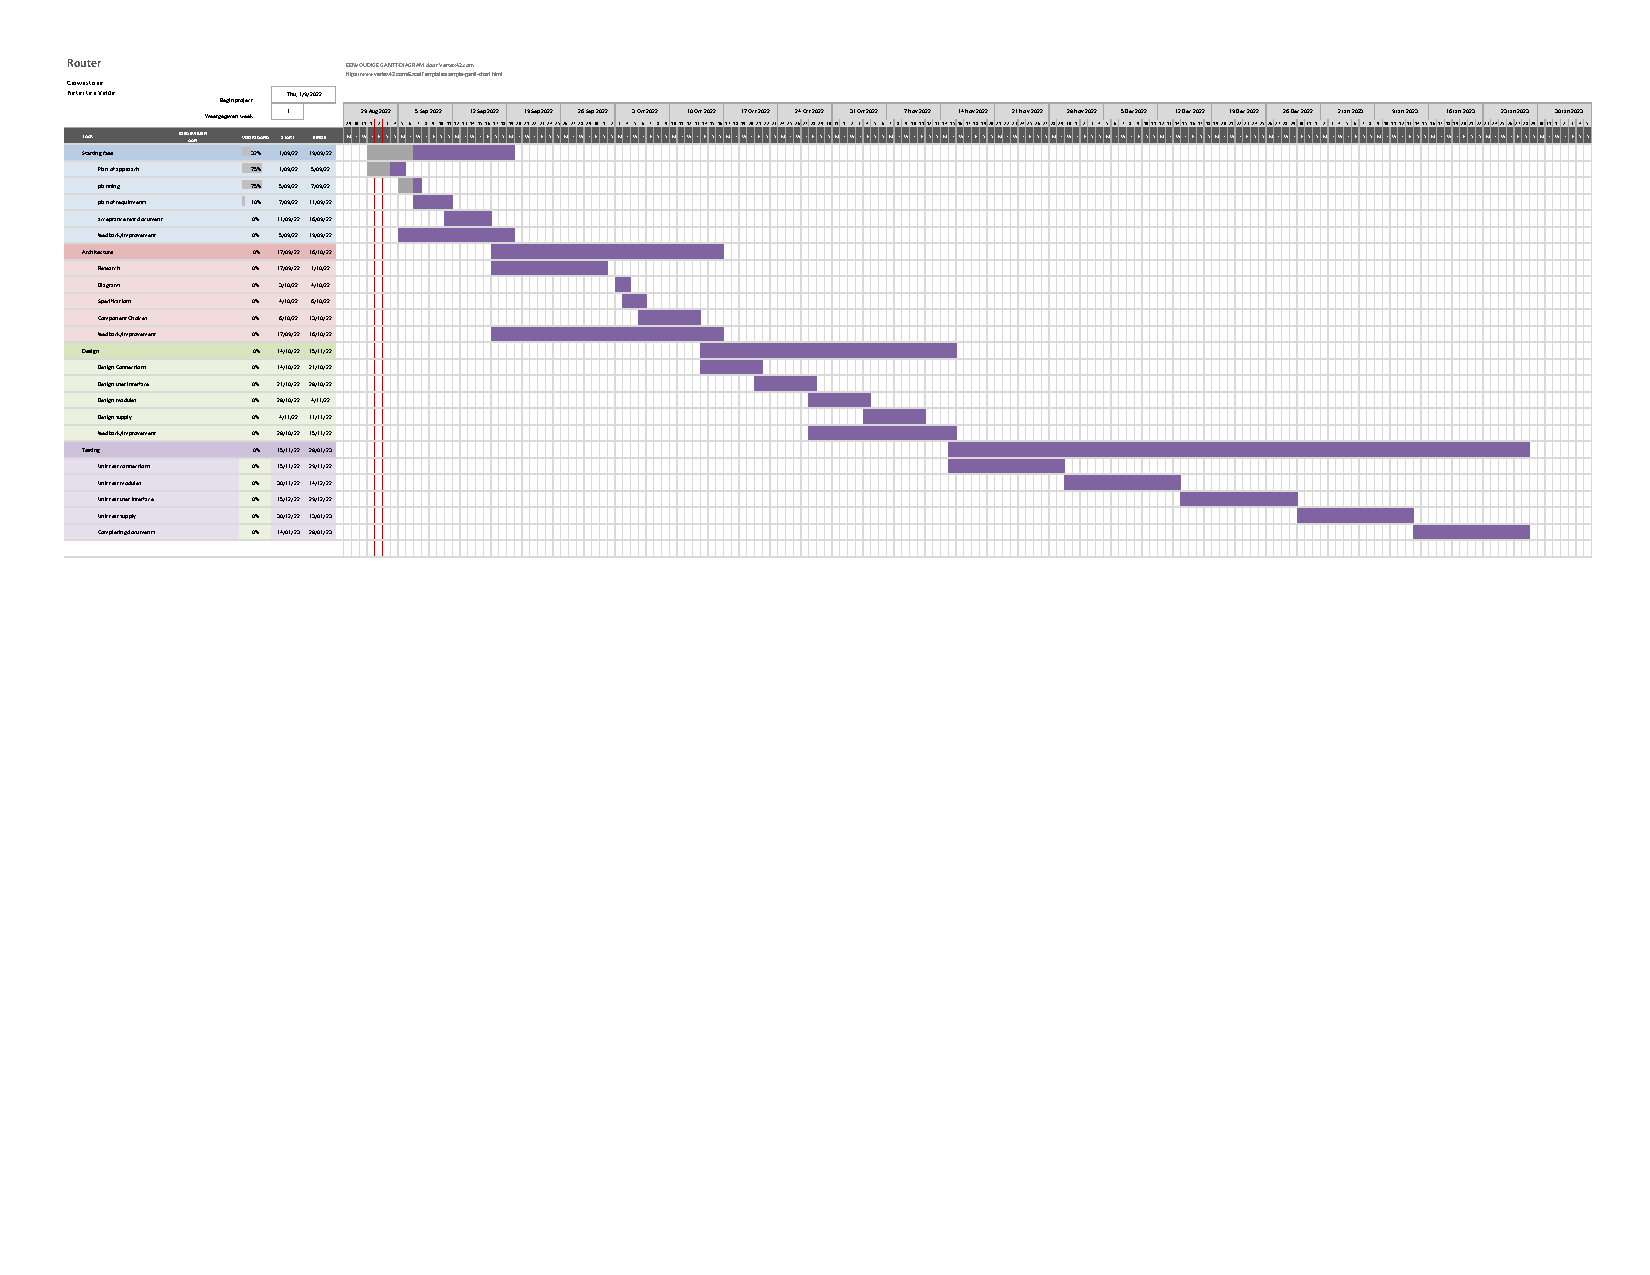
\includepdf[pages={1},angle=90]{Planning_POA.pdf}
\end{landscape}

\end{document}